\section{Umsetzung}
\label{sec:Umsetzung}

Nachdem die Entwurfsphase abgeschlossen wurde kann  mit der Umsetzung der
Anwendung begonnen werden. In der Phase der Projektumsetzung werden hierbei
zwei Teilphasen unterschieden werden, welche weitestgehend unabhängig
voneinander ablaufen: Zum einen muss die eigentliche Anwendung realisiert
werden. Zum anderen müssen die 360-Grad Panoramas erstellt werden, welche den
späteren Hauptinhalt der Anwendung darstellen. Im Nachfolgenden sollen beide
Teilphasen näher untersucht und die einzelnen Teilschritte innerhalb der Phasen
verdeutlicht werden. Dieser Einblick in die Projektdurchführung soll Aufschluss
über die Funktionsweise der zu erstellenden Anwendung und der bei der
Realisierung verwendeten Technologien bieten.

\subsection{Panoramaerstellung}
\label{sec:Panoramaerstellung}

\subsubsection{Anforderungen an die Panoramafotos}
\label{sec:PanoramaerstellungAnforderungen}

Die Panoramaerstellung stellt, neben der Softwareerstellung einen zentralen
Teilprozess innerhalb der Projektumsetzung dar. Bevor mit der Erstellung der
Panoramas begonnen werden kann müssen zunächst die Anforderungen der Anwendung
an die Panoramafotos festgelegt werden. Hierbei muss definiert werden, welche
Kriterien die Panoramafotos erfüllen müssen, um von der Anwendung korrekt
verarbeitet werden zu können. Relevante Kriterien sind hierbei die
Darstellungsform, die Größe und das Format der Panoramafotos. Nachdem diese
Schnittstelle festgelegt ist kann der Prozess der Panoramaerstellung isoliert
vom Prozess der Softwareerstellung durchgeführt werden. Dies ermöglicht eine
parallele Umsetzung der beiden Teilprozesse.

Wie bereits in \verweis{Architektur} erwähnt soll in der Anwendung die Google
Street View API verwendet werden. Diese Schnittstelle stellt die Funktionalität
zur Anzeige der Panoramafotos zur Verfügung. Somit legt diese Schnittstelle auch
fest, in welcher Form die Panoramafotos zur Verfügung gestellt werden müssen.
Diese Anforderungen können aus der Entwicklerdokumentation zu der API entnommen
werden. Die Schnittstelle erwartet hierbei ein Panoramafoto, welches der
Rektangulatprojektion\footnote{Die Rektangularprojektion stellt eine
horizontale Ansicht von 360 Grad und eine vertikale Ansicht von 180 Grad dar.
Dies bedingt ein Seitenverhälnis von 2:1} entspricht. Durch die API wird diese
Darstellung auf die Fläche einer Kugel projeziert. Der Mittlepunkt dieser Kugel
stellt den Standpunkt des Betrachters dar. Da sich immer nur ein Teil der
Projektion im Blickfeld dieses Betrachters befindet muss auch nur der aktuell
sichtbare Bereich des Panoramafotos dargestellt werden. Aus diesem Grund bietet
die Google Street View API die Möglichkeit, ein in mehrere rechteckige Teile,
sogenannte Kacheln, aufgeteiltes Panoramafoto zu verarbeiten. Auf diese Weise
kann die Performanz der Anwendung erhöht werden, da nicht das komplette
Panoramafoto, sondern nur ein Teil der Kacheln in der Anwendung geladen werden
muss. Damit den einzelnen Kacheln die korrekte Position auf der Planarprojektion
zugewiesen werden kann, muss die Benennung der Kacheldateien dem Namensschema
\texttt{Kachelspalte-Kachelzeile} genügen. Die Anzahl der Kacheln sowie die
Pixelmaße des Panoramafotos können frei gewählt werden. Hierbei ist zu beachten,
dass mit steigender Pixelanzahl die Qualität der 360-Grad-Darstellung steigt,
die Performance der Anwendung jedoch aufgrund der steigenden Datengröße sinkt.
In einer prototypischen Implementierung, auf die im \verweis{Softwareerstellung}
näher eingegangen werden soll, hat die Projektgruppe verschiedene Kombinationen
aus Pixekmaße und Kachelanzahl getestet. Letztendlich hat sich die Projektgruppe
auf die Pixelmaße 4096x2048 für das gesamte Panorama und eine Aufteilung in 32
Kacheln entschieden. Diese Kombination wurde einheitlich als bester Kompromiss
zwischen Qualität und Performanz angesehen.
\subsubsection{Workflow der Panoramaerstellung}
\label{sec:Workflow}

Der Workflow der Panoramaerstellung kann in mehrere Teilprozesse untergliedert
werden. Für die Umsetzung dieser einzelnen Teilschritte wird hierbei spezielles
Hard- und Softwareequipment benötigt. Im Folgenden sollen die einzelnen
Teilschritte der Panoramaerstellung in chronologischer Reihenfolge erläutert
werden. Im Zuge dessen soll auch auf das benötigte Equipment eingegangen
werden.

\paragraph{Aufnahme der Einzelfotos} \hfill \\

Die Panoramaerstellung beginnt mit der Aufnahme mehrerer Einzelfotos. Aus diesen
Einzelfotos wird nachfolgend dann das komplette Panoramafoto zusammengefügt.
Dieses muss, wie zuvor erläutert, der Rektangularprojektion entsprechen. Die
Summe der Einzelfotos muss also eine horizontale Ansicht von 360 Grad und eine
vertikale Ansicht von 180 Grad abbilden. Die Anzahl der Einzelfotos ist somit
von dem Bildwinkel abhängig, der auf einem einzelnen Foto dargestellt werden
kann. Dieser Bildwinkel wird in der Fotografie durch die Brennweite des
Objektives festgelegt. Je geringer die Brennweite eines Objektives ist, desto
größer ist der Bildwinkel, der mit diesem Objektiv eingefangen werden kann und
desto weniger Einzelfotos werden für die Erstellung eines Panoramafotos
benötigt. Durch spezielle Objektivkonstruktionen wie zum Beispiel einem
Fisheye-Obektiv ist es möglich einen besonders großen Bildwinkel aufzunehmen.
Ein solches Objektiv und eine zum dem Objektiv kompatible Kamera wird auch für die Aufnahme der
Panoramafotos im Projekt verwendet. Das Objektiv ermöglicht es in 16 Fotos alle
Ansichten Aufzunehmen, die zur Darstellung einer Rektangularprojektion benötigt
werden. In 15 dieser Einzelfotos ist hierbei die horizontale Rundumansicht
dargestellt. Das sechzehnte Foto bildet den Zenit\footnote{Der Zenit ist der
Punkt über dem Beobachter/der Kamera} im Panoramafoto ab. Der
Nadir\footnote{Der Nadir ist der dem Zenit gegenüber gelegene Punkt unter dem
Beobachter/der Kamera} wird in den Panoramafotos nicht abgebildet, da sich hier
das Stativ befindet.

Zur Unterstützung bei der Aufnahme hat sich die Projektgruppe weiterhin
entschieden ein speziell für die Panoramafotografie ausgelegtes Stativ zu
verwenden. Eine Aufnahme ohne dieses Stativ wäre zwar denkbar, würde die
Qualität der Panoramafotos jedoch stark beeinträchtigen. Das Panoramastativ
besteht aus folgenden Komponenten:

\begin{description}
\item[Stativ] Das eigentliche Stativ dient dazu, die Kamera im Raum an einer
festen Position zu fixieren. Hierdurch ist sichergestellt, dass alle
Einzelfotos von der selben Position aus aufgenommen werden.
\item[Nivelliervorrichtung] Die Nivelliervorrichtung dient dazu, den Kopf des
Statives horitontal auszurichten. Auf diese Weise wird ein wellenförmiger
Horizont in dem zusammengefügten Panoramafoto vermieden.
\item[Rotator] Der Rotator ermöglicht es, den Kopf des Stativs um die vertikale
Achse zu drehen. Weiterhin kann eine Gradzahl festgelegt werden, nachdem der
Mechanismus bei einer Drehnung einrastet. Auf diese Weise wird eine gleichmäßige
Drehung bei der Aufnahme der Panoramafotos ermöglicht.
\item[Nodalpunktadapter] Der Nodalpunktadapter ermöglicht es, die Kamera auf
dem Stativ so zu positionieren, dass die Eintrittspupille des Stativs auf Höhe
der vertikalen Drehachse des Stativs liegt. Hierdurch können
Parallaxenfehler\footnote{Der Parallaxenfehler beschreibt eine scheinbare
Verschiebung zweier hintereinandergelegener Gegenstände, wenn sich der
Ausgangspunkt der Betrachtung ändert} bei der Aufnahme vermieden werden
\end{description}

Das komplette Equipment, welches zur Aufnahme der Panoramafotos verwendet wurde,
ist in \abbildung{Equipment} dargestellt.

\begin{figure}[htb]
\centering
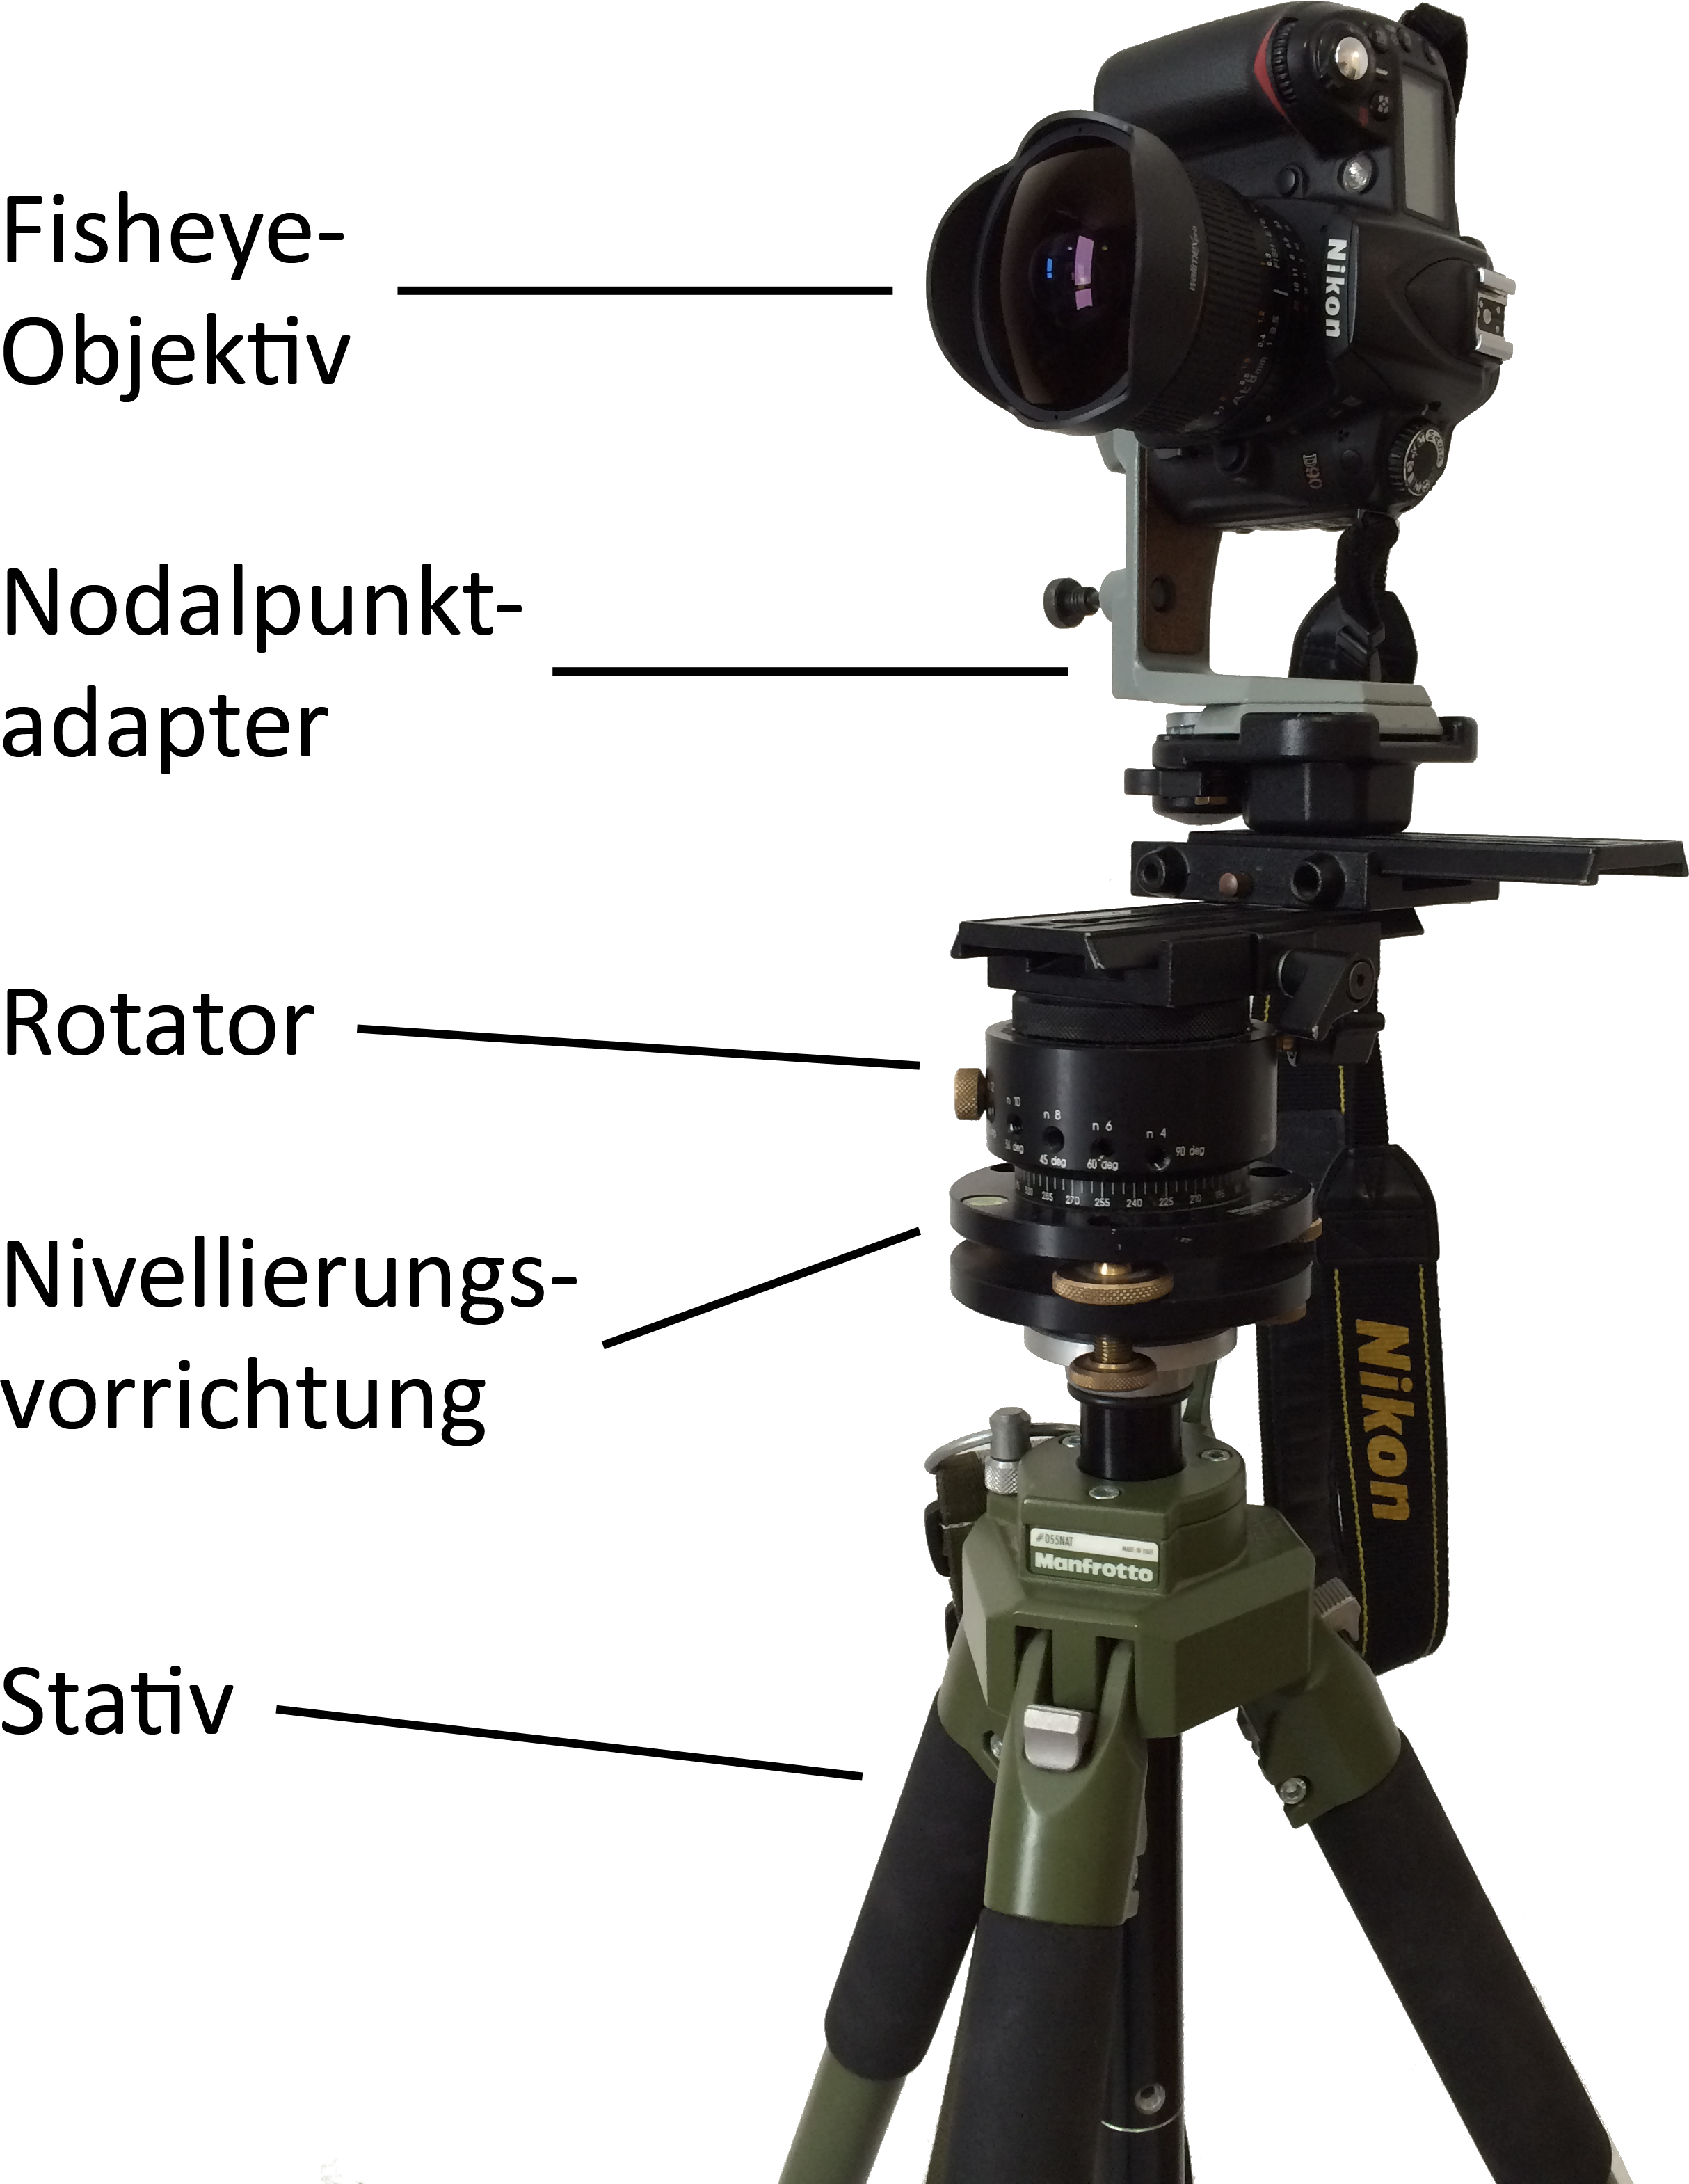
\includegraphics[width=0.5\textwidth]{Equipment.png}
\caption[Equipment zur Aufnahme der Einzelfotos]{Equipment zur Aufnahme der Einzelfotos\protect\footnotemark}
\label{fig:Equipment}
\end{figure}
\footnotetext{Eigene Darstellung}

\clearpage

\paragraph{Stitching und Rendering} \hfill \\

Nachdem die Einzelfotos aufgenommen wurden müssen diese zu einem Panoramafoto
zusammengefügt werden. Dieser Prozess wird als Stitching bezeichnet. Das
Stitching erfolgt im Projekt mit der Software Kolor Autopano Giga 3.0. Die
Software ist in der Lage, die Einzelfotos automatisiert zusammenzufügen.
Gegebenenfall muss das hieraus resultierende Panoramafoto nach dem
automatisierten Zusammenfügen noch manuell ausgerichtet werden. Aufgrund
dieser manuellen Ausrichtung ist es nicht möglich, den hier beschriebenen
Prozess vollständig zu automatisieren. In einem letzen Schritt wird das
zusammengefügte Panoramafoto dann in das JPEG-Format konvertiert. Dieser Schritt
wird als Rendering bezeichnet. Das Ergebnis dieses Prozesses ist in
\abbildung{Zusammengefuegt} dargestellt.

\begin{figure}[htb]
\centering
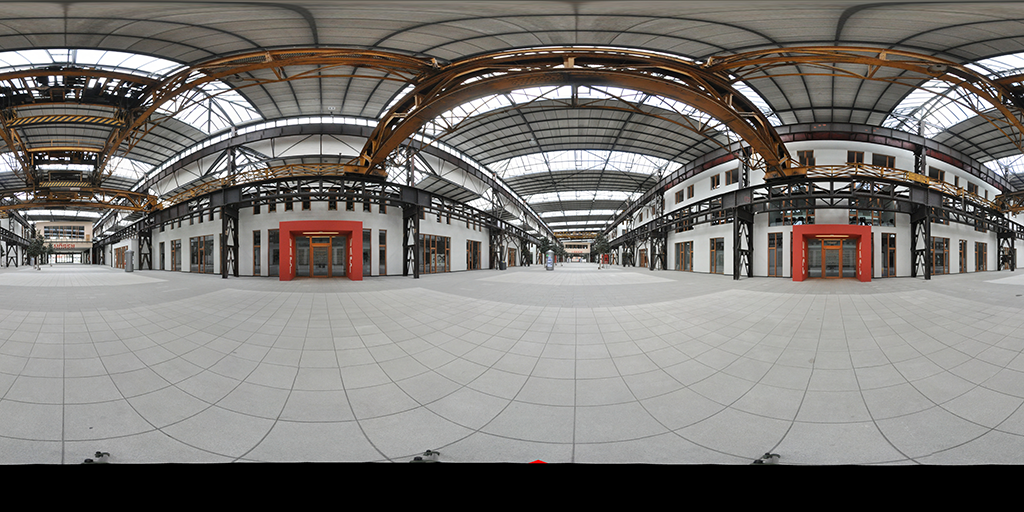
\includegraphics[width=0.8\textwidth]{Zusammengefuegt.png}
\caption[Panoramafoto nach Stitching und Rendering]{Panoramafoto nach Stitching
und Rendering\protect\footnotemark}
\label{fig:Zusammengefuegt}
\end{figure}
\footnotetext{Eigene Darstellung}

\paragraph{Überarbeitung und Optimierung der Panoramafotos} \hfill \\

Da es bei der Aufnahme der Einzelfotos nicht möglich war den Nadir abzubilden,
fehlen diese Informationen folglich auch in dem zusammengefügten
Pa\-no\-ra\-ma\-fo\-to. In \abbildung{Zusammengefuegt} ist der Bereich, in dem
die Bildinformationen fehlen, durch eine schwarze Fläche markiert. Im Zuge
einer Überarbeitung der Panoramafotos soll dieser schwarze Bereich mit einem
Label überdeckt werden, auf dem das Logo des Projektes dargestellt ist. Das
Label muss dabei so verzerrt werden, dass es nach der bereits beschriebenden
Projezierung durch die Google Street View API entzerrt dargestellt ist.

Neben der Überarbeitung der Panoramafotos werden diese weiterhin für die
Darstellung im Internet optimiert. Hierbei wird die Größe des Panoramafotos auf
die Pixelmaße 4096x2048 reduziert und die JPEG-Datei komprimiert abgesspeichert.

Die Bearbeitung der Panoramafotos erfolgt mit der Software Adobe Photoshop CS5.
Durch die Stapelverarbeitungsfunktion des Programms können alle hier
beschriebenen Teilschritte automatisiert durchgeführt werden. Das Ergebnis
dieses Prozesses ist in \abbildung{Ueberarbeitet} dargestellt.

\begin{figure}[htb]
\centering
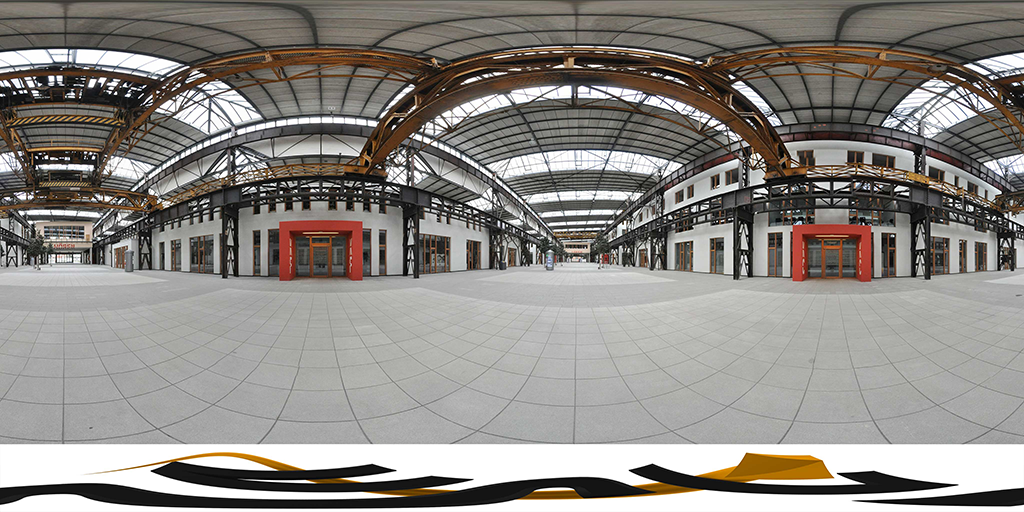
\includegraphics[width=0.8\textwidth]{Ueberarbeitet.png}
\caption[Panoramafoto nach Überarbeitung und Optimierung]{Panoramafoto nach
Überarbeitung und Optimierung\protect\footnotemark}
\label{fig:Ueberarbeitet}
\end{figure}
\footnotetext{Eigene Darstellung}

\paragraph{Aufteilung des Panoramafotos in Kacheln} \hfill \\

Das Blickfeld des Benutzers in der Anwendung nimmt immer nur einen Teil der
Rundumansicht ein. Somit kann auch immer nur ein Teil des Panoramafotos
dargestellt werden. Es ist daher nicht sinnvoll das komplette Panoramafoto in
der Anwendung zu laden, bevor es dem Benutzer präsentiert wird.
Aus diesem Grund wird das Panoramafoto in einem letzten Bearbeitungsschritt in
mehrere Kacheln aufgeteilt. Ziel dieser Aufteilung ist eine Steigerung der
Performanz und eine Reduzierung der Ladezeiten für die Panoramafotos in der
Anwendung. Es muss immer nur der Teil der Kacheln geladen werden, der dem
Benutzer aktuell präsentiert wird. Wenn sich das Blickfeld des Benutzers ändert,
können einzelne Kacheln schnell nachgeladen werden.

Die Aufteilung der Panoramafotos im Projekt erfolgt, wie auch die Überarbeitung
der Fotos, mit der Software Adobe Photoshop CS5. Auch hier kann die
Stapelverarbeitungsfunktion genutzt werden, um die Aufteilung der Panoramafotos
zu automatisieren.

\subsection{Softwareerstellung}
\label{sec:Softwareerstellung}

Die zu erstellende Software erfüllt die Anforderungen des Lastenheftes, in dem die Modelle und Konzepte der Entwurfsphase implementiert werden. Die Umsetzung eines solchen Projektes mit einem mehrköpfigem Projektteam erfordert neben entsprechenden Softwareentwürfen auch Vorbereitung und den Einsatz spezieller Entwicklungswerkzeuge (Tools), die im nachfolgenden Abschnitt beschrieben sind.

\subsubsection{Vorbereitung und Tools}
\label{sec:VorbereitungUndTools}

Die besondere Herausforderung des vorliegenden Projektes besteht darin, eine
mehrschichtige Software, bestehend aus Benutzer- und Administrationsansicht, in
einem Projektteam zu entwickeln, welches sich in zwei Punkten von der
Projektorganisation eines klassischen\footnotemark\ Softwareprojektes
unterscheidet. Zum einem muss  as Projektteam, bedingt durch unterschiedliche
Arbeitsorte, räumlich getrennt voneinander entwicklen können. Zum anderen
ist das Projektteam während des Entwicklungszeitraums nicht vollständig im
Projekt eingebunden. Es müssen Arbeits-, Urlaubs-, Prüfungs- und
Krankheitszeiten aller Mitglieder des Projektteams als hemmende Zeitfaktoren
berücksichtigt werden. Eine genauere Betrachtung dieser Projektsituation ist an
dieser Stelle nicht notwendig.

\footnotetext{Klassische Softwareprojekte werden hier als Projekte
in einer reinen Projektorganisation verstanden. Zur weiteren Vertiefung siehe
\citet[S.~105]{jenny2001}}

Die beiden genennten Aspekte bergen organisatorische Risiken und können auch zu
Problemen bei der Entwicklung führen. Das Hauptrisiko ist dabei ein Stillstand
des Projektes, welcher dadurch bedingt ist, dass alle Projektmitglieder auf das
Wissen eines Mitglieds angewiesen sind, welches gerade nicht zur Verfügung
steht. Dieses Risiko soll durch den Einsatz von zwei Entwicklungswerkzeugen
minimiert werden.

Zunächst muss dafür gesorgt werden, dass alle Mitglieder immer auf dem
aktuellen Stand des Projektes sind. Wird ein Entwicklungsschritt von einer
einzelnen Person abgeschlossen muss das Ergebnis den anderen zur Verfügung
gestellt werden. Zusätzlich müssen Änderungen am bestehnden Projektstand
kommentiert und dokumentiert werden. Diese Anforderung werden im vorliegenden
Projekt mithilfe einer Projektversionierung erreicht. Ein Versionierungstool
bietet hierbei die Möglichkeit den Quellcode eines Softwareprojektes zentral in
einem sogenannten Repository (zu deutsch "`Depot"') zu halten, um ihn für alle
Mitglieder verfübgar zu machen. Der aktuelle Stand des Projektes kann aus
diesem Repository jederzeit abgefragt werden und Änderungen werden von
Mitgliedern dorthin zurückgeschrieben. Zusätzlich bieten Versionierungstools die
Möglichkeit, die Änderung mit einem Kommentar zu versehen. Die Dokumentation der
konkrteten Änderungen wird vom Tool automatisch durchgeführt. Als
Versionierungssoftware wurde im vorliegenden Projekt "`Github"'\footnotemark\
verwendet, da allen Mitglieder mit diesem Versionierungstool bereits gearbeitet
haben.

\footnotetext{Github ist eine Open Source Projekt, das auf dem
Versionierungstool git aufsetzt. Es stellt den De-facto-Standard für
Webprojekte dar.}

Neben dem Quellcode sollen auch die Anforderungen an die Anwendung und die
aktuellen Aufgaben der Projektmitglieder an zentraler Stelle verwaltet werden.
Bei Ausfall eines Mitgliedes müssen seine aktuellen Aufgaben zentral
dokumentiert sein, um diese auf andere Mitglieder verteilen zu können. Dazu
wurde ein webbasiertes Ticketsystem aufgesetzt, auf das alle Mitglieder zugriff
haben. Hierbei wurde sich für das Ticketsystem "`PHProjekt"' entschieden, da PHP
als Technologie bereits bekannt ist und das Ticketsystem somit schnell
aufgesetzt werden konnte. In diesem Ticketsystem werden alle erstellten
Arbeitspakete des Projektes mit zugeordnetem Mitglied, Bearbeitungszeitraum,
Anforderungsbeschreibung und benötigter Bearbeitungszeit hinterlegt.
\subsubsection{Prototyp}
\label{sec:Prototyp}

Nach Bereitstellung des Ticketsystems und des Versionierungstools kann mit der Implementierung der Software begonnen werden. Für die Auftraggeber des Projektes war es dabei besonders wichtig, dass zunächst ein Prototyp der späteren Software entwickelt wird. Dieser Prototyp sollte nur die 360 Grad Ansicht eines Campus Panoramas und die Möglichkeit zu einem weiteren Panorama zu navigieren enthalten. Der Prototyp sollte genutzt werden um Entscheidungsträger von Beginn an vom Projekt zu überzeugen.

Da der Prototyp nur einen statischen Einblick (kein dynamischer Inhalt aus einer Datenbank) in die späteren Benutzeransicht gewähren sollte, wurde hierfür ein HTML-Dokument geschrieben, das die Google Street View API einbindet und über Javascript dessen Funktionalität implementiert. Das erstellte HTML-Dokument ist in \listing{HTML Prototyp} dargestellt:

\lstinputlisting[language=HTML,caption={HTML Prototyp},label={lst:HTML Prototyp}]{Listings/HTML_Prototyp.html}

Das dargestellte HTML-Dokument bindet in Zeile 5 die angesprochene Google Street View API, in der Funktionen zur Darstellung des 360 Grad Panoramas definiert sind. Zusätzlich wird in Zeile 6 eine Javascript-Datei eingebunden, in der die Funktionen der Google Street View API auferufen werden. Im Body-Bereich des HTML-Dokumentes ist dafür ein Element definiert das als Fläche zur Darstellung der Panoramas genutzt wird. Die eingebundene Javascript-Datei aus Zeile 6 ist aus Platzgründen in \listing{Javascript Prototyp} in Anhang ~\ref{sec:AnhangJavascriptPrototyp} dargestellt. Dessen Funktionalität wird an dieser Stelle kurz erläutert.
%TODO: Anhang XX richtig einfügen

Sobald der Internetbrowser des Benutzers das HTML-Dokument fertig geladen hat, wird eine Methode aufgerufen, die benötigte Parameter zur Erstellung des Panoramas bereitstellt\footnote{Vergleiche Zeile 3 im Anhang XX}. Hier werden Zoomstufe, Ausrichtung und weitere Parameter festgelegt. Anschließend wird ein Panorama-Objekt mit Hilfe der Google Street View API erstellt und an das oben beschriebene HTML-Element im Body-Bereich gebunden\footnote{Vergleiche Zeile 16-18 im Anhang XX}. Über einen weiteren Aufruf einer API-Funktion können an das Panorama sogenannte "`Links"' gehängt werden. Diese Links stellen später für den Benutzer die Pfeile am Boden dar über die zu anderen Panoramas navigiert werden kann. Im Prototyp wird nur der Verweis auf ein anderes Panorama gebraucht, das über die Funktion "`createCustomLinks"'\footnote{vergleiche Zeile 45ff. im Anhang XX} als Link angehängt wird.

Ein Bildschirmfoto des Prototypen der mitt diesen zwei Dateien (HTML- und Javascript-Dokument) erstellt wurde ist in \abbildung{PrototypScreenshot} zu sehen.

%TODO: Screenshot ohne Pixelfehler machen!
\begin{figure}[htb]
\centering
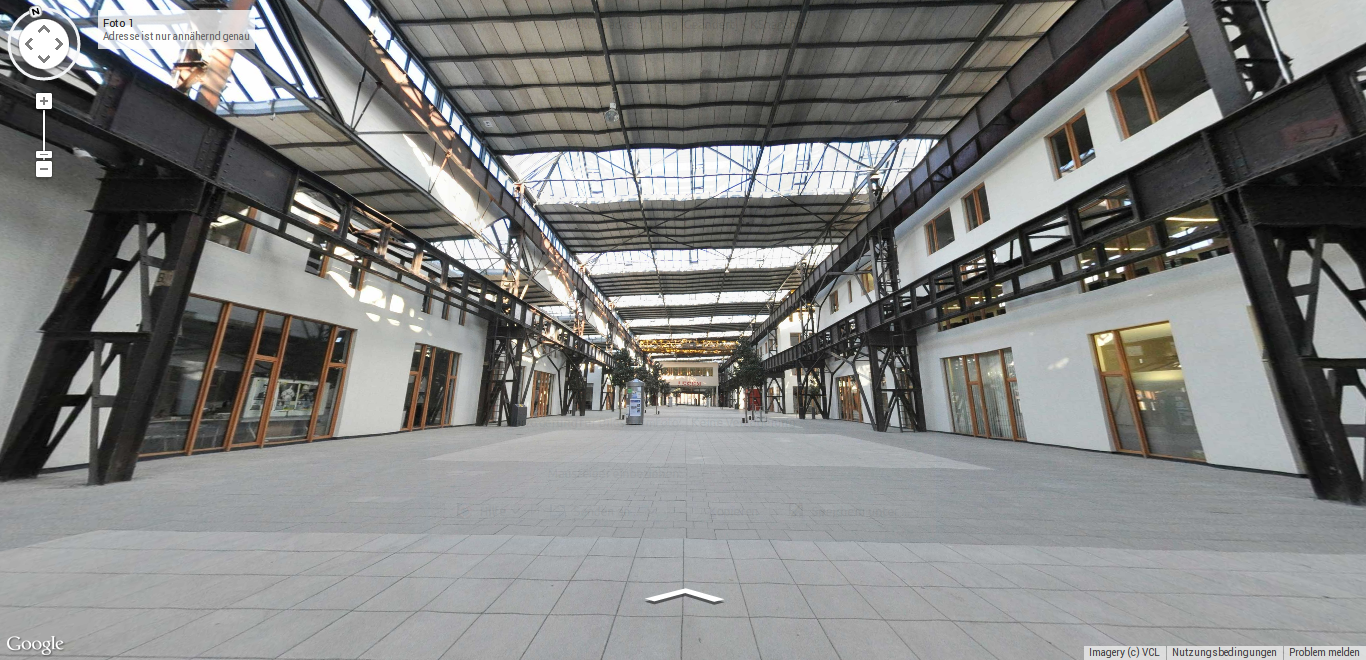
\includegraphics[width=1.0\textwidth]{PrototypScreenshot.png}
\caption[PrototypScreenshot]{Bildschirmfoto des Prototypen}
\label{fig:PrototypScreenshot}
\end{figure}
\subsubsection{Administrationsbereich}
\label{sec:UmsetzungAdministrationsbereich}

Der entwickelte Prototyp stellt eine erste lauffähige Version einer Benutzeransicht dar. Der nächste Entwicklungsschritt ist die Implementierung des Administrationsbereiche und die Bereitstellung von APIs. Aufbauend auf gepflegten Ìnformationen im Administrationsbereich wird der Prototyp dann um dynamische Funktionalität erweitert. Das heißt die angezeigten Panoramas und die benachbarten Panoramas werden über eine API angefragt, die die Informationen aus der Datenbank lädt. Der Implementierungsprozess des Administrationsbereiches wird dabei sukzessiv anhand der vorgestellten Anwendungsfällen (siehe \nameref{sec:Adminstratoranwendungen} auf Seite \pageref{sec:Adminstratoranwendungen}) realisiert. Prioresiert werden dabei die Anwendungsfälle, die die Verwaltung der Panoramas, Infotexte und die Übersichtskarte betreffen (AFA05 bis AFA17).

Bevor mit der Implementierung begonnen werden kann wird noch ein einheitliches Design festgelegt, dass vor allem dem späteren Administrator das Verständnis erleichtert. Zu diesem einheitlichen Design Konzept zählt zum Beispiel das Farbschema von Buttons. So wurde beispielsweise festgelegt, dass ein roter Button immer das Löschen eines Datensatzes signalisiert und ein grüner immer das speichern eines Datensatzes. Darüber hinaus wurde entschieden die Gestaltung von Buttons, Informationsfenster und ähnlichem mit dem CSS\footnotemark\ Framework Bootstrap\footnotemark\ zu realisieren. Dadurch ist gewährleistet, dass alle Steuerungselemente in allen Browsern gleich aussehen und der Administrator Elemente durch ihr Aussehen wiedererkennen und darüber auf ihre Benutzung schließen kann. Durch diese Entscheidungen wird die Usability der Software erhöht und der Aufwand der zu erstellenden Dokumentation verringert.

\footnotetext{CSS steht für Cascading Style Sheets und beschreibt eine Skriptsprache, die dazu dient HTML-Elemente in Form und Farbe zu verändern.}

\footnotetext{Bootstrap ist ein open Source Projekt, in dem einheitlich das Design von verschiedenen HTML-Elemente definiert ist. Bootstrap ist ein Projekt des Internetkonzerns Twitter und ist besonders dafür geeignet ein einheitliches Look and Feel einer Webseite in allen Browsern zu erzeugen.}

Aufbauend auf Administratoranwendungsfällen und Designkonzept werden Tickets erstellt, deren Inhalt die Implementierung der Infotext- und Fotoverwaltung ist. Zur Verdeutlichung der eingesetzten Technologien und des Entwicklunsablaufs wird im Folgenden eine stark vereinfachte Fotoverwaltungsseite implementiert. Implementiert werden soll eine Seite, die alle Fotos der Datenbank mit Namen und Beschreibung anzeigt. Zustätzlich soll es dem Administrator möglich sein auf den Namen eines Fotos zu klicken, woraufhin ihm weitere Informationen angezeigt werden.

Zur Implementierung dieses Szenarios wird zunächst ein HTML-Dokument angefertigt, dass das Grundgerüst der Fotoverwaltung darstellt. In diesem Grundgerüst könnten bestimmte Elemente, wie zum Beispiel die Navigationsbar am oberen Rand (vergleiche \abbildung{MockupBackend}) der Seite oder der Titel der Seite, statisch codiert werden. Zur Vereinfachung soll aber nur der Titel der Seite gesetzt werden und eine Überschrift. Das folgende \listing{HTML_Anwendungsbeispiel} zeigt das angefertigte HTML-Dokument.

\lstinputlisting[language=HTML,caption={statisches HTML},label={lst:HTML_Anwendungsbeispiel}]{Listings/HTML_Anwendungsbeispiel.html}

Im Anschluss daran muss die Seite um dynamisch generierten Inhalt erweitert werden. Dynamischer Inhalt ist im gegeben Anwendungsfall das Anzeigen aller Fotos, die bereits in der Datenbank sind. Um dieses Verhalten zu realisieren muss eine Anfrage an die Datenbank gestellt werden und danach muss für jeden Eintrag in der Datenbank HTML Quellcode geschrieben werden. Das nachfolgende \listing{HTML mit PHP} zeigt die Implementierung mit PHP.

\lstinputlisting[language=HTML,caption={Dynamisches schreiben von HTML mit PHP},label={lst:HTML mit PHP}]{Listings/HTML_mit_PHP.php}

Zu sehen ist die Anfrage an die Datenbank, die durch die PHP-Funktion "`mysql\_query"' (Zeile 5) realisiert wird, das Durchlaufen jeden Datenbanksatzes in einer Schleife (Zeile 6ff.) und das schreiben von HTML mit dem PHP "`echo"'-Befehl.

Zum Abschluss wird das klicken auf den Fotonamen implementiert. Diese Benutzerinteraktion kann am besten auf dem Clientsystem des Benutzers (Internetbrowser) mit Javascript verarbeitet werden, da keine weiteren Informationen vom Server benötigt werden und zusätzliche Anfragen so vermieden werden. Javascript-Routinen werden meistens als Funktionen formuliert, die aufgerufen werden, wenn ein bestimmtes Ereignis eintritt. Im \listing{HTML mit PHP} ist ein solcher Funktionsaufruf in Zeile 9 zu sehen. Die Funktion "`toggleDescription"' wird aufgerufen sobald auf das <p>-Tag geklickt wird. Als Parameter wird dieser Funktion das eigene HTML-Element, also das <p>-Tag, mitgegeben. Die Javascript-Funktion ist in \listing{Javascript Snippet} dargestellt.

\lstinputlisting[language=JavaScript,caption={Auf Benutzerinteraktion reagieren mit Javascript},label={lst:Javascript Snippet}]{Listings/Javascript_Snippet.js}

Alle dargestellten Listings könnten dabei in einem Dokument stehen, das vom dem Administrator über seinen Internetbrowser angefragt wird.
Wie bereits erwähnt ist diese Darstellung der Implementierung sehr stark vereinfacht. Die Quelldateien, die die Fotoverwaltung im vorliegenden Projekt implementieren, sind zu umfangreich, um sie an dieser Stelle zu präsentieren. Die implementierte Fotoverwaltung wird in folgendem Bildschirmfoto zur Veranschaulichung dargestellt:

%TODO: Bildschirmfoto ohne Pixelfehler machen.
\begin{figure}[htb]
\centering
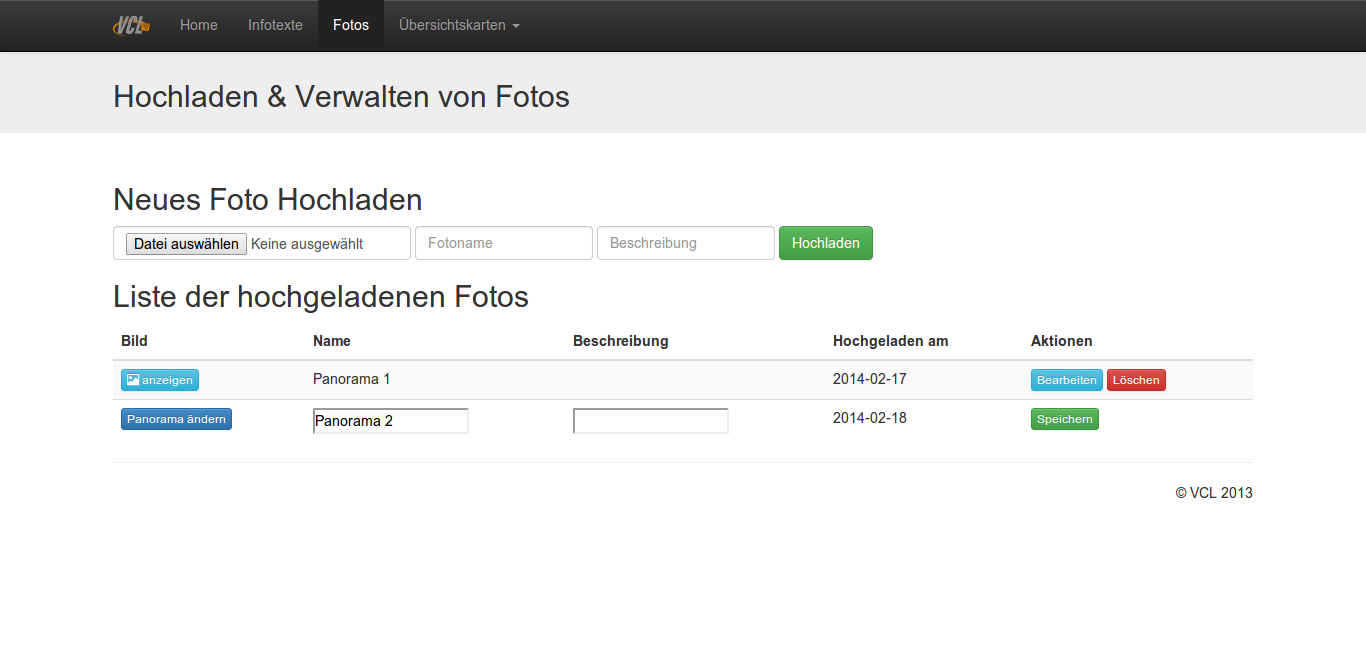
\includegraphics[width=1.0\textwidth]{Fotoverwaltung.png}
\caption[Fotoverwaltung]{Bildschirmfoto der implementierten Fotoverwaltung}
\label{fig:Fotoverwaltung}
\end{figure}

In einem solchen Entwicklungszyklus wurde auch die Verwaltung der Infotexte und die Übersichtskarte implementiert. Bildschirmfotos dieser Bereiche sind im Anhang dargstellt, siehe \abbildung{ScreenshotInfotext}, \abbildung{ScreenshotUebersichtskarte}.
\subsubsection{Application Programming Interfaces (APIs)}
\label{sec:APIs}

Aufbauend auf dem abgeschlossen Administrationsbereich werden im Folgenden
Application Programming Interfaces, kurz APIs, implementiert. Aufgabe solcher
APIs ist es, Informationen in maschinenleserlicher Form für andere Teilbereiche
des Systems bereitzustellen. Die bereitgestellten Informationen werden von den
aufrufenden Systemen genutzt, um Inhalte dynamisch darzustellen.
In einem Beispiel soll der zuvor vorgestellte Prototyp die Menge der
benachbarten Panoramas über eine solche API beziehen und darauf aufbauend dem
Benutzer die Navigationspfeile entsprechend präsentieren. Die Implementierung
einer API wird nachfolgend an diesem Beispiel erläutert.

Die Realisierung der Schnittstelle vollzieht sich in zwei Schritten.
Zuerst werden die Informationen maschienenleserlich geschrieben und ausgeben. Im
zweiten Schritt werden diese Informationen dann von einem verarbeitenden System
eingelesen und ausgewertet. Das Schreiben von maschinenleserlichen Informationen
hängt stark davon ab, welche Maschine den ausgegeben Text lesen bzw.
interpretieren soll. Im vorliegenden Projekt werden die erstellten APIs
ausschließlich von Javascript-Routinen angefragt, um Inhalte asynchron
nachzuladen. Auf die Bedeutung von asynchronem Nachladen wird später genauer
eingegangen. An dieser Stelle ist lediglich zu beachten, dass die APIs von
Javascript-Routinen angefragt werden. Aus diesem Grund werden die Informationen
der API im JSON-Format dargestellt. JSON steht dabei für "`Javascript Object
Notation"' und ist der de facto Standard für die Kommunikation zwischen
webbasierten Schnittstellen.\footnote{\citet[S.~20]{lubbers2011}} Die
Darstellung im JSON-Format bietet den großen Vorteil, dass innerhalb von
Javascript aus den dargestellten Informationen ein Objekt im Sinne der
objektorientierten Programmierung\footnotemark erstellt werden kann. An dieser
Stelle soll diese Begründung für die Wahl des JSON-Formats ausreichen. Eine
genauere Betrachtung erfolgt im zweiten Schritt der Implementierung der API.
Neben der Klassifikation der API muss noch der darzustellende Inhalt definiert
werden. Für den oben beschriebenen Anwendungsfall müssen hierbei alle Nachbarn
eines gegebenen Panoramas dargestellt werden. Für die Ausrichtung der
Navigationspfeile wird zusätzlich die Himmelsrichtung in Grad jedes Nachbarn
relativ zum Standpunkt des gegeben Panoramas benötigt. Dieser letzte Wert wird
als "`Heading"' bezeichnet und wird bereits bei der Positionierung des
360-Grad-Fotos in der Datenbank gespeichert. Er muss also nur aus der Datenbank
abgefragt werden.

\footnotetext{Die Objektorientierte Programmmierung (OOP) ist
das führende Programmierparadigma für Webanwendungen. Dieses Paradigma
beschreibt eine bestimmte Denkweise für Problemstellungen der Informatik. Für
weitere Einblicke siehe \citet{poetzsch2000}}

Aufbauend auf der vorausgegangenen Beschreibung der API kann diese in PHP
implementiert werden. Dazu wird zunächst das in \verweis{Datenbankentwurf}
beschriebene Tabellenmodell in Bezug auf die darzustellenden Informationen
untersucht. In der \abbildung{Tabellenmodell} ist zu sehen, dass
\textit{heading} ein Attribut der Tabelle \textit{neighbour} ist. Über diese
Tabelle können zu einem gegeben Panorama alle Nachbarn mit entsprechendem
\textit{heading} gefunden werden.
Im Zuge der Implementierung sollen im Folgenden mit Hilfe von PHP über SQL alle
Nachbarn eines gegebenen Panoramas abgefragt werden. Das Ergebnis dieser
Abfrage soll im JSON-Format dargestellt werden. Im \listing{PHP_Nachbar_API}
ist diese Funktionalität implementiert.

\lstinputlisting[language=PHP,caption={PHP Nachbar
API},label={lst:PHP_Nachbar_API}]{Listings/PHP_Nachbar_API.php}

Das gebene Panorama wird im Listing über die aufrufende URL, also einem
HTTP\footnotemark -Parameter, gesetzt. In der URL
\url{http://vcl.example.com/api/api\_test.php?id=1} würde beispielsweise der
Parameter id ("`?id=1"') mit der Panorama-ID 1 übergeben werden. Das
Auslesen dieser Information ist im Listing in Zeile 2 dargestellt.
Unter der Annahme, dass das Panorama mit der ID 1 zwei Nachbarn hat, würde der
Aufruf der API folgendes Ergebnis liefern:

\footnotetext{HTTP steht für Hypertext Transfer Protocol und bezeichnet ein
Protokoll, das den Übertragungsstandard für Webdokumente darstellt. HTTP stellt
damit eine fest protokollierte Struktur auf, in der geregelt ist, wie ein
Dokument über das Internet übertragen wird.}

\clearpage

\begin{figure}[htb]
\centering
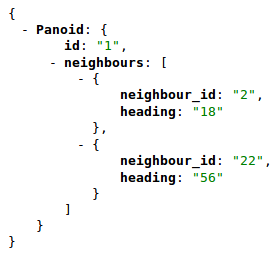
\includegraphics[width=0.4\textwidth]{ScreenshotAPIBeispiel.png}
\caption[API Beispiel]{Bildschirmfoto des gegebenen API Beispiels}
\label{fig:ScreenshotAPIBeispiel}
\end{figure}

Die Darstellung dieser Ausgabe wurde mit Hilfe eines Darstellungstools auf
bessere Lesbarkeit optimiert. Im Normalfall würde die Ausgabe in einer Zeile
dargestellt werden. Dies zeigt wiederum, dass das Ausgabeformat nicht auf
menschliche Lesbarkeit ausgelegt ist.

Nachdem das ausgebende System der Beispielschnittstelle implementiert wurde,
soll dieses nachfolgend angefragt und die Antwort des Systems ausgewertet
werden. Die Anfrage an das System erfolgt, wie bereits erwähnt, asynchron
innerhalb einer Javascript-Funktion. Asynchron bedeutet hierbei, dass die
Anfrage unabhängig von dem Aufbau der restlichen Seite ausgeführt wird.
Unabhängig von der aktuell dargestellten Seite wird eine Anfrage ausgeführt,
dessen Ergebnis in die bereits dargestellte Seite integriert wird.

In \verweis{Prototyp} wurde bereits die Funktion "`createCustomLink"' aus dem
Anhang ~\ref{sec:AnhangJavascriptPrototyp}
(\nameref{sec:AnhangJavascriptPrototyp}) vorgestellt. In dieser Funktion
werden die Links festgelegt, die letzenendes die Navigationspfeile in der
Benutzeransicht abbilden. Im \verweis{Prototyp} wurden diese Links statisch
gesetzt. Nachfolgend soll der Prototyp in der Weise abgeändert werden, dass die
Links durch Aufrufen der API dynamisch festgelegt werden. Dazu wird die Funktion
\textit{createCustomLink} zunächst um einen Funktionausruf der Funktion
"`getPanoJson"' erweitert. Diese Funktion ist dafür zuständig, die oben
definierte API mit einer übergebenen ID anzufragen und ein JSON-Objekt an die
aufrufende Methode zurückzuliefern. Die Implementierung dieser Funktion ist in
\listing{Dynamisch_Nachbarn_nachladen} dargestellt.

\clearpage

\lstinputlisting[language=JavaScript,caption={Dynamisch Nachbarn
nachladen},label={lst:Dynamisch_Nachbarn_nachladen}]{Listings/Dynamisch_Nachbarn_nachladen.js}

Die Funktion \textit{getPanoJson} wird in Zeile 5 aufgerufen und fragt daraufhin
über einen sogenannten \textit{XMLHttpRequest} die oben genannte URL an (Zeile
25). Da die Antwort als unformartiertes Textdokument erfolgt und es nicht
möglich ist per HTTP Objekte zu übertragen muss die Antwort zunächst in ein
JSON-Objekt umgewandelt werden. Man spricht dabei von "`parsen"' (Zeile 28). Die
Elemente des zurückgelieferten JSON-Objektes (Zeile 30) können daraufhin von der
aufrufenden Funktion referenziert werden. Über "`pano.neighbours"' (Zeile 7)
erhält man beispielsweise eine Liste aller Nachbarn, die im oben dargestellten
Quellcode durchlaufen und in die \textit{Links}-Liste geschrieben werden (Zeile
8ff.).

Durch die Erweiterung des Prototyps ist dieser in der Lage, die im
Administrationsbereich gepflegten Daten dynamisch abzurufen.

An dieser Stelle des Entwicklungsprozesses sind die Funktionen des
Administrationsbereichs vollständig umgesetzt und die Benutzeransicht greift
über APIs dynamisch auf die hinterlegten Informationen zu. Die Umsetzung des
Projektes ist damit abgeschlossen.
